\section{Combinatoria}

Dado un conjunto $C$ de $n$ elementos distinguibles, ¿cuantas formas hay de elegirlos para formar conjuntos de $p$ elementos?

\begin{center}
	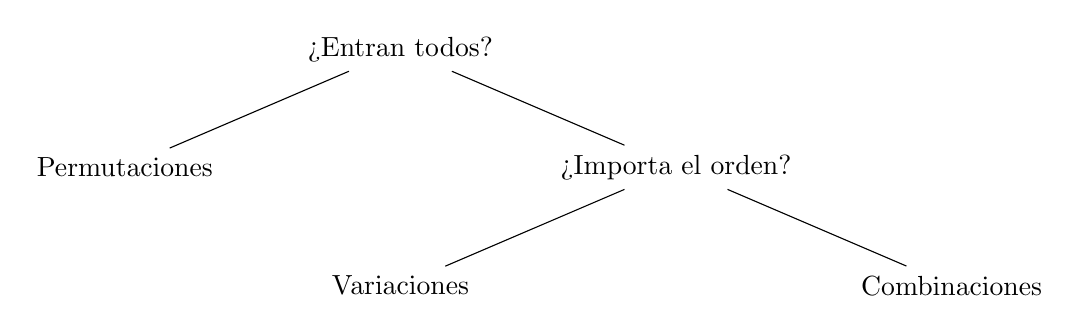
\begin{tikzpicture}[sibling distance=70mm]
		\node {¿Entran todos?}
		child {node {Permutaciones}}
		child {node {¿Importa el orden?}
		child {node {Variaciones}}
		child {node {Combinaciones}}
		};
	\end{tikzpicture}
\end{center}

\begin{tabular}{c|c|c}
	Permutaciones & Variaciones & Combinaciones \\
	\hline
	\begin{tabular}{c|c}
		Sin    & Con \\
		$\text{P}_n = n!$ & $\text{PR}^n_{n_1,\cdots,n_k}=\frac{n!}{n_1!\cdots n_k!}$
	\end{tabular} & \begin{tabular}{c|c}
		                Sin                      & Con \\
		                $\text{V}^n_p = \frac{n!}{(n-p)!}$ & $\text{VR}^n_p = n^p$
	\end{tabular} & \begin{tabular}{c|c}
		                Sin                & Con  \\
		                $\text{CR}^n_p =  \binom{n}{p}$ & $\text{C}^n_p = \binom{n+p-1}{p}$
	\end{tabular}
\end{tabular}

\subsection{Variaciones}

\begin{example}
	¿Cuántas banderas diferentes de tres franjas horizontales de colores distintos pueden confeccionarse a
	partir de siete colores diferentes?

	Tenemos un conjunto $C$ de $n=7$ colores distintos, y por tanto distinguibles, y queremos elegirlos para formar elementos de $C^3$, el número de elementos distintos es
	\[
		\text{V}^7_3=\frac{7!}{(7-3)!}=\frac{7!}{4!}=7*6*5=210
	\]
\end{example}

\begin{example}
	¿Cuántas quinielas de 14 resultados distintas se pueden rellenar?

	Tenemos un conjunto $C=\set{1, x, 2}$ de $n=3$ elementos y tenemos que formar elementos de $C^{14}$.
	\[
		\text{VR}^{3}_{14} = 3^{14}=4782969
	\]
\end{example}

\subsubsection{Permutaciones con repetición}
Podemos formar $k$ grupos indistinguibles de cardinales $n_1,\cdots, n_k\tq \sum_{i=1}^k n_i=n$.


\begin{example}
	¿Cuántos números de seis cifras se pueden formar con los dı́gitos 1, 2 y 3?

	Se trata de determinar el número de ordenaciones distintas de un conjunto de seis elementos formados por tres
	grupos distintos de elementos indistinguibles, $\set{1, 1, 1}, \set{2, 2}, \set{3}$.
	\[
		\text{PR}^6_{3,2,1}=\frac{6!}{3! 2! 1!}=60
	\]
\end{example}

\subsection{Combinaciones}

\begin{example}
	Un estudiante debe responder a seis de las diez preguntas de las que consta un examen, ¿cuantas formas distintas tiene de hacer el examen?

	Se trata de determinar el número de grupos distintos de seis preguntas escogidas del conjunto de las diez, sabiendo que dos grupos con las mismas preguntas, aún en distinto orden, coinciden.
	En este caso, el número de grupos de preguntas distintos entre los que se puede elegir es
	\[
		\text{C}^{10}_6 = \begin{pmatrix*}
			                  10\\6
		\end{pmatrix*} =\frac{10!}{6!(10-6)!}=\frac{10!}{6!4!}=\frac{10*9*9*7}{4*3*2}=210
	\]
\end{example}

\begin{example}
	¿De cuántas formas pueden elegirse simultáneamente tres bolas de una urna en la que hay al menos tres bolas bolas blancas y tres negras indistinguibles?

	Cada grupo es una disposición no ordenada de tres colores formada por los colores blanco y negro con repetición de alguno de ellos.
	Por tanto, se trata de determinar el número de grupos de tres elementos no ordenados del conjunto {b, n}.
	En este caso, el número de formas distintas de elegir simultáneamente tres bolas del conjunto es
	\[
		\text{CR}^2_3=\begin{pmatrix*}
			              4\\3
		\end{pmatrix*} =\frac{4!}{3!1!}=4
	\]
\end{example}